%!TEX root=../main.tex

\section{Problem Setup}
\label{sec:setup}

The setup of our framework most follows the \emph{Equalized Odds}
framework \cite{hardt2016equality,zafar2017fairness}; however, we extend their framework for use with
probabilistic classifiers.
Let $P \subset \R^k \times \{0, 1\}$ be the input space of a binary classification task.
In our criminal justice example, $\left( \x, y \right) \sim P$ represents a person, with
$\x$ representing the individual's history and $y$ representing whether or not the person
will commit another crime.
%
Additionally, we assume the presence of two groups
$G_1, G_2 \subset P$,
which represent disjoint population subsets, such as different races.
We assume that the groups have different \emph{base rates} $\br_{t}$, or probabilities
of belonging to the positive class:
%
$
\br_{1} = \Pr_{(\x, y) \sim G_1} \left[ y = 1 \right] \neq \Pr_{(\x, y) \sim G_2} \left[ y = 1 \right] = \br_{2}.
$

%
Finally, let $h_1, h_2 : \R^k \rightarrow [0, 1] $ be binary classifiers,
where $h_1$ classifies samples from $G_1$ and $h_2$ classifies samples from $G_2$.\footnote{
In practice, $h_1$ and $h_2$ can be trained jointly (i.e. they are the same classifier).}
Each classifier outputs the probability that a given sample $\x$ belongs to the positive class.
The notion of Equalized Odds non-discrimination is based on the false-positive
and false-negative rates for each group, which we generalize here for use with probabilistic
classifiers:
%
\begin{definition}
  \label{def:fpfn}
  The \emph{generalized false-positive rate} of classifier $h_t$ for group $G_t$ is
  %
  $
  \fp{h_t} = \ev_{(\x, y) \sim G_t} \bigl[ h_t(\x) \mid y\!=\!0 \bigr].
  $
  %
  Similarly, the \emph{generalized false-negative rate} of classifier $h_t$ is
  %
  $
    \fn{h_t} = \ev_{(\x, y) \sim G_t} \bigl[ \left( 1 - h_t(\x) \right) \mid y\!=\!1 \bigr].
  $
\end{definition}
%
If the classifier were to output either $0$ or $1$, this represents
the standard notions of false-positive and false-negative rates.
We now define the Equalized Odds framework (generalized for probabilistic classifiers),
which aims to ensure that errors of a given type are not biased against
any group.
%
\begin{definition}[Probabilistic Equalized Odds]
  \label{def:eo}
  Classifiers $h_1$ and $h_2$ exhibit Equalized Odds for groups $G_1$
  and $G_2$ if $\fp{h_1} = \fp{h_2}$ and $\fn{h_1} = \fn{h_2}$.
\end{definition}
%
%

\paragraph{Calibration Constraints.}
%
As stated in the introduction, these two conditions do not necessarily prevent
discrimination if the classifier predictions do not represent well-calibrated
probabilities.
%\footnote{
  %Note that such discrimination can still occur even when a classifier outputs
  %non-probabilistic scores. \gp{Expand on this}
%}
Recall that calibration intuitively says that
probabilities should carry semantic meaning:
if there are 100 people in $G_1$ for whom
$h_1(\x) = 0.6$, then we expect $60$ of them to belong to the positive class.
%
\begin{definition}
  \label{def:calibration}
  A classifier $h_t$ is \emph{perfectly calibrated} if $\forall p \in [0, 1]$,
  $\Pr_{(\x, y) \sim G_t} \bigl[ y\!=\!1 \mid h_t(\x)\!=\!p \bigr] = p$.
\end{definition}
%
It is commonly accepted amongst practitioners that both classifiers $h_1$ and $h_2$
should be calibrated \emph{with respect to groups} $G_1$ and $G_2$ to prevent
discrimination \cite{berk2017fairness,crowson-calibration-risk-scores,dieterich-northpointe-fairness,flores-re-propublica-fair}.
Intuitively, this prevents the probability scores from carrying group-specific
information.
Unfortunately, \citet{kleinberg2016inherent} (as well as
\cite{chouldechova2017fair}, in a binary setting) prove that
a classifier cannot achieve both calibration and Equalized Odds, even in an approximate
sense, except in the most
trivial of cases.

\subsection{Geometric Characterization of Constraints}

We now will characterize the calibration and error-rate constraints with
simple geometric intuitions. Throughout the rest of this paper, all of our
results can be easily derived from this interpretation.
%
We begin by defining the region of classifiers which are \emph{trivial}, or
those that output a constant value for all inputs (i.e. $h^{c}(\x) = c$,
where $0 \leq c \leq 1$ is a constant).
We can visualize these classifiers on a graph with generalized false-positive
rates on one axis and generalized false-negatives on the other.
It follows from the definitions of generalized false-positive/false-negative
rates and calibration that all trivial classifiers $h$ lie on the diagonal defined by
$\fp{h} + \fn{h} = 1$ (\autoref{fig:calibration}).
Therefore, all classifiers that are ``better than random'' must lie below this
diagonal in false-positive/false-negative space (the gray triangle in the figure).
Any classifier that lies above the diagonal performs
``worse than random,'' as we can find a point on the trivial classifier diagonal
with lower false-positive and false-negative rates.

Now we will characterize the set of calibrated classifiers for groups $G_1$ and $G_2$, which
we denote as $\mathcal{H}^*_1$ and $\mathcal{H}^*_2$.
\citeauthor{kleinberg2016inherent} show that the generalized false-positive and
false-negative rates of a calibrated classifier are
linearly related by the base rate of the group:\footnote{
  Throughout this work we will treat the calibration constraint as holding
  exactly; however, our results generalize to approximate settings as well. See the
  Supplementary Materials for more details.
}
%
\begin{equation}
  \fn{h_t} = (1 - \br_t) / \br_t \: \fp{h_t}.
\end{equation}
%
In other words, $h_1$ lies on
a line with slope $(1 - \br_1) / \br_1$ and
$h_2$ lies on a line with slope $(1 - \br_2) / \br_2$ (\autoref{fig:calibration}).
The lower endpoint of each line is the \emph{perfect classifier}, which
assigns the correct prediction with complete certainty to every input.
The upper endpoint is a trivial classifier, as no calibrated classifier
can perform ``worse than random'' (see \autoref{lma:trivial} in
\autoref{app:cost-funcs}).
The only trivial classifier that satisfies the calibration
condition for a group $G_t$ is the one that outputs the base rate $\mu_t$.
We will refer to $h^{\br_1}$ and $h^{\br_2}$ as the trivial classifiers,
calibrated for groups $G_1$ and $G_2$ respectively.
It follows from the definitions that $\fp{h^{\br_1}} = \mu_1$
and $\fn{h^{\br_1}} = 1 - \mu_1$, and likewise for $h^{\br_2}$.

Finally, it is worth noting that for calibrated classifiers,
a lower false-positive rate necessarily corresponds to a lower false-negative rate
and vice-versa.
In other words, for a given base rate, a ``better'' calibrated classifier
lies closer to the origin on the line of calibrated classifiers.
%(This also holds in an approximate sense; see \autoref{sec:cost_and_error}.)


\paragraph{Impossibility of Equalized Odds with Calibration.}
%
With this geometric intuition, we can provide a simplified
proof of the main impossibility
result from \cite{kleinberg2016inherent}:
%
\begin{thm*}[Impossibility Result \cite{kleinberg2016inherent}]
  \label{thm:orig-impossibility}
  Let $h_1$ and $h_2$ be classifiers for groups $G_1$ and $G_2$ with $\br_1 \neq \br_2$.
  $h_1$ and $h_2$ satisfy the Equalized Odds and calibration conditions
  if and only if $h_1$ and $h_2$ are perfect predictors.
\end{thm*}
%
Intuitively, the three conditions define a set of classifiers which
is overconstrained.
Equalized Odds stipulates that the classifiers $h_1$ and
$h_2$ must lie on the same coordinate in the false-positive/false-negative
plane. As $h_1$ must lie on the blue line of calibrated classifiers for $\mathcal{H}_1^*$ and $h_2$ on the red line $\mathcal{H}_2^*$ they can only satisfy EO at the unique intersection point --- the origin (and location of the perfect classifier).
% The only point thatd
% satisfies this constraint as well as the calibration constraint is where the
% two calibration lines intersect, which is the origin.
This implies that unless the two classifiers achieve perfect accuracy,
we must relax the Equalized Odds conditions if we want to
maintain calibration.


\begin{figure}[t]
  \centering
  \begin{subfigure}[b]{0.22\textwidth}
    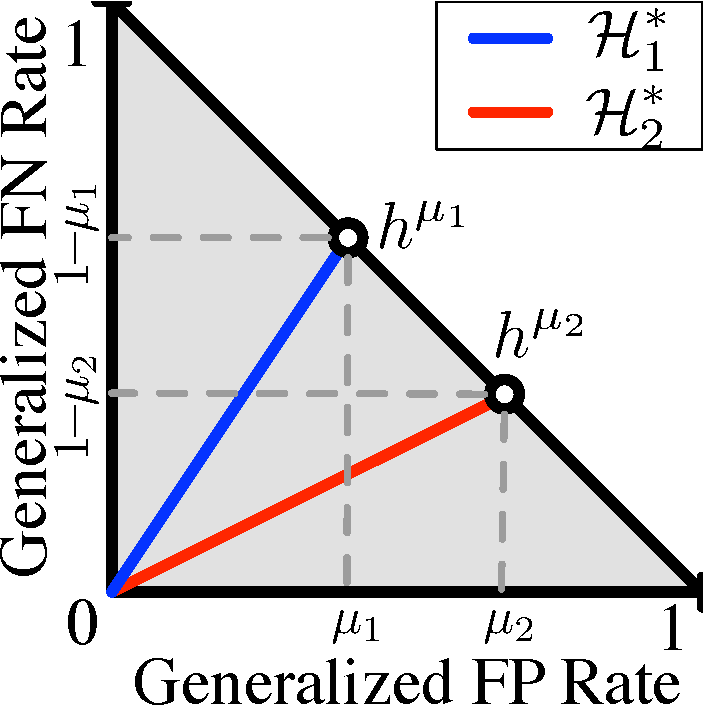
\includegraphics[width=\textwidth]{figures/calibrated.pdf}
    \caption{Possible cal. classifiers $\mathcal{H}^*_1, \mathcal{H}^*_2$ (blue/red).}
    \label{fig:calibration}
  \end{subfigure}
  \quad
  \begin{subfigure}[b]{0.22\textwidth}
    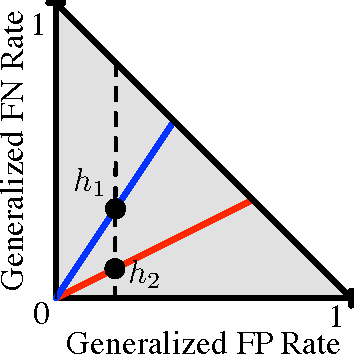
\includegraphics[width=\textwidth]{figures/calibrated-fp.pdf}
    \caption{Satisfying cal. and equal F.P. rates.}
    \label{fig:two-of-three-fp}
  \end{subfigure}
  \quad
  \begin{subfigure}[b]{0.22\textwidth}
    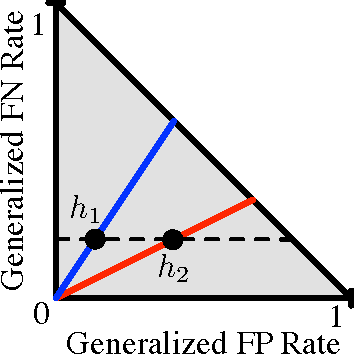
\includegraphics[width=\textwidth]{figures/calibrated-fn.pdf}
    \caption{Satisfying cal. and equal F.N. rates.}
    \label{fig:two-of-three-fn}
  \end{subfigure}
  \quad
  \begin{subfigure}[b]{0.22\textwidth}
    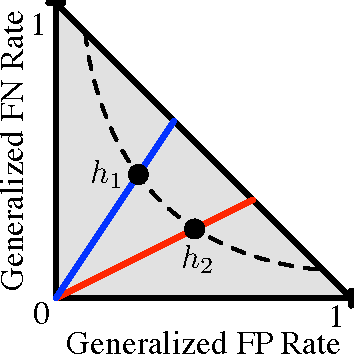
\includegraphics[width=\textwidth]{figures/calibrated-general.pdf}
    \caption{Satisfying cal. and a general constraint.}
    \label{fig:general-disparity}
  \end{subfigure}
  \caption{
  Calibration, trivial classifiers, and equal-cost constraints -- plotted in the
  false-pos./false-neg. plane.
  $\mathcal{H}^*_1, \mathcal{H}^*_2$ are the set of cal. classifiers for the two groups, and $h^{\mu_1}, h^{\mu_2}$ are trivial classifiers.
  }
  \label{fig:two-of-three-conditions}
\end{figure}
\begin{figure}[t]
  \centering
  \begin{subfigure}[b]{0.22\textwidth}
    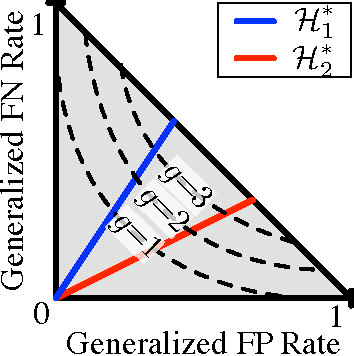
\includegraphics[width=\textwidth]{figures/level-order-curves.pdf}
    \caption{Level-order curves of cost. Low cost implies low
      error rates.}
    \label{fig:levelorder}
  \end{subfigure}
  \quad
  \begin{subfigure}[b]{0.22\textwidth}
    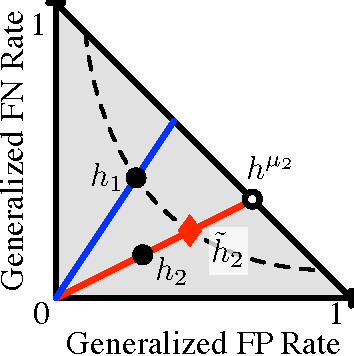
\includegraphics[width=\textwidth]{figures/post-process.pdf}
    \caption{Usually, there is a calibrated classifier $\tilde h_2$ with the same cost of $h_1$.}
    \label{fig:postprocess}
  \end{subfigure}
  \quad
  \begin{subfigure}[b]{0.22\textwidth}
    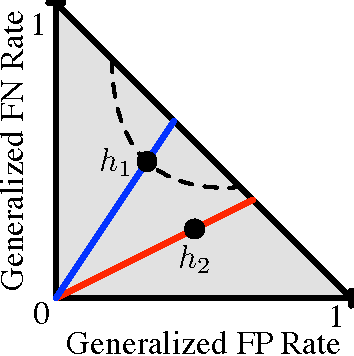
\includegraphics[width=\textwidth]{figures/infeasible.pdf}
    \caption{Cal. and equal-cost are incompatible
    if $h_1$ has high error.}
    \label{fig:infeasible-trivial}
  \end{subfigure}
  \quad
  \begin{subfigure}[b]{0.22\textwidth}
    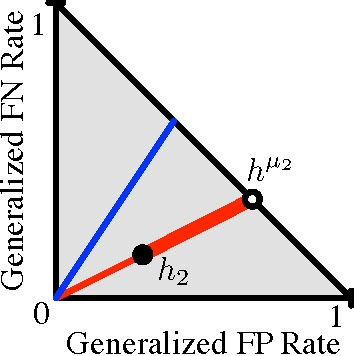
\includegraphics[width=\textwidth]{figures/interp.pdf}
    \caption{Possible cal. classifiers for $G_2$ (bold red) by
    mixing $h_2$ and $h^{\mu_2}$.}
    \label{fig:mixing}
  \end{subfigure}
  \caption{
    Calibration-Preserving Parity through interpolation.
  }
  \label{fig:feasible}
\end{figure}
